\subsection{Loop} \label{subsec:loop}

\subsubsection*{Allgemein}

\begin{figure}
\centering
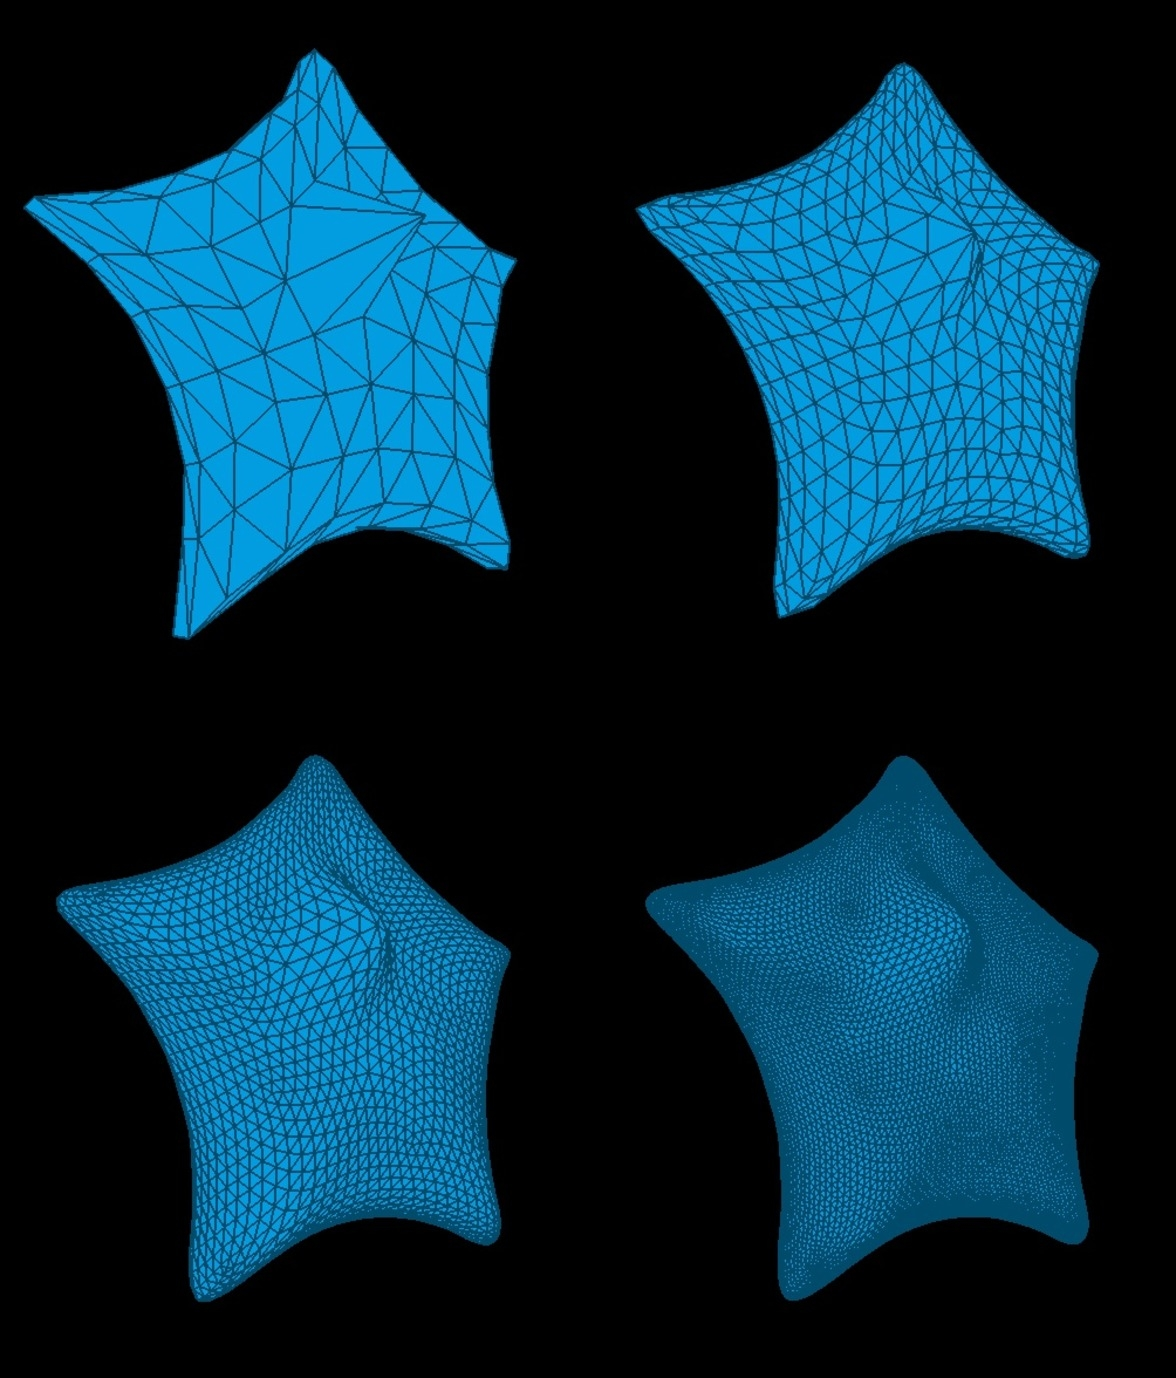
\includegraphics[width=0.8\textwidth]{content/media/cc5_edge_loop.jpg}
\caption{Drei Unterteilungsschritte mit dem Loop Algorithmus}
\label{fig:sd_loop_cc5}
\end{figure}

Charles Loop hat 1987 einen Unterteilungsalgorithmus für Dreiecksnetze entwickelt.
Der Loop Algorithmus basiert auf quartischen Box Splines und approximiert die Kontrollpunkte.
An extraordinären Stellen mit Valenz ungleich sechs erzeugt Loop \(C^1\) stetige Flächen,
im regulären Fall \(C^2\).
\autoref{fig:sd_loop_cc5} zeigt drei Unterteilungsschritte.
\cite[S. 70 f.]{Zorin.subdivcourse} \cite[S. 56 f.]{Standford.24.07.2015}

\subsubsection*{Unterteilungs- und Randregeln}

Die Unterteilung erfolgt in drei Schritten.
\begin{enumerate}
\item Berechne für jede Kante einen Edge Point. Dieser wird auch als Odd Vertex bezeichnet.
\item Berechne für jeden Vertex eine neue Position. Dieser wird auch als Even Vertex bezeichnet.
\item Ersetze jedes Dreieck durch vier neue Dreiecke.
\end{enumerate}

\autoref{fig:sd_loop_mask} zeigt die Masken für die Unterteilung
und für Randfälle.
Entlang des Randes (boundary/crease) wird eine kubische Spline Kurve erzeugt.
\cite[S. 70]{Zorin.subdivcourse}
\begin{figure}
\centering
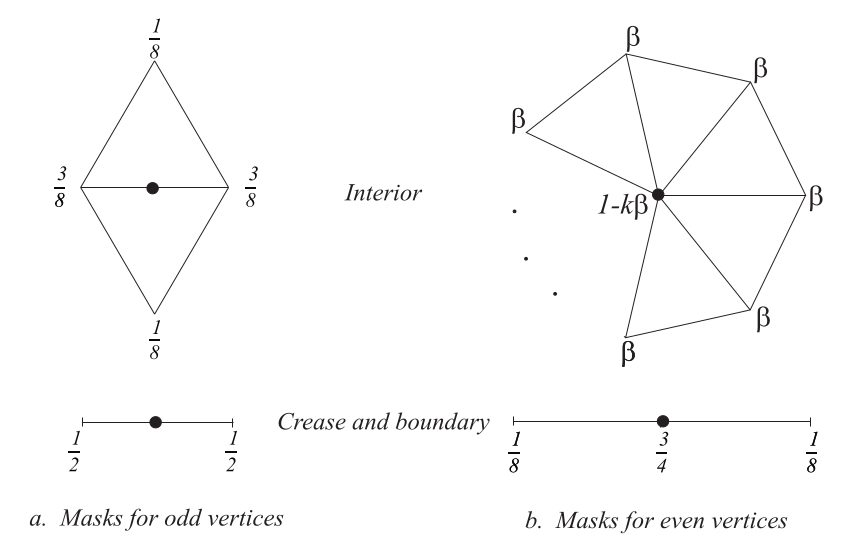
\includegraphics[width=1.0\textwidth]{content/media/sd_loop_mask.jpg}
\caption{Loop Maske \cite[S. 70 f.]{Zorin.subdivcourse}}
\label{fig:sd_loop_mask}
\end{figure}

\paragraph*{Odd Vertex}
Die Odd Vertices werden nach der linken Maske aus \autoref{fig:sd_loop_mask} berechnet.
Für Ränder wird der Mittelwert errechnet.

\paragraph*{Even Vertex}

Bei Even Vertices muss für die Berechnung der Faktor \(\beta\) bestimmt werden.
\autoref{fig:sd_loop_mask} veranschaulicht auf der rechten Seite die Berechnung.
Der Even Vertex wird nach der Bestimmung von \(\beta\) wie folgt berechnet werden:\\
\(
even\_vertex = old\_vertex \cdot (1 - k \cdot \beta) + sum\_of\_surrounding\_vertices \cdot \beta\\
k:\ Valenz
\)
\\
Für die Bestimmung von \(\beta\) gibt es mehrere Möglichkeiten:
\begin{description}
\item[Original nach Loop]  \(\beta=\frac{1}{k}(\frac{5}{8}-(\frac{3}{8}+\frac{1}{4} \cdot cos(\frac{2\pi}{k}))^2)\)
\item[Variation nach Warren] \mbox{}
	\begin{itemize}
		\item für \(k > 3,\ \beta = \frac{3}{8k}\)
		\item für \(k = 3,\ \beta = \frac{3}{16}\)	
	\end{itemize}
\end{description}
Die Variation nach Warran hat den Vorteil, dass diese einfacher berechnet werden kann
und somit eine perfomantere Implementierung möglich ist.
Die Variante nach Warren ist auch in SubVis implementiert.

Für Ränder muss \(\beta\) nicht bestimmt werden.
Hier kann das einfache Schema aus \autoref{fig:sd_loop_mask} angewendet werden.
\cite{Carnegie}
\cite{Standford.Loop}
\cite[S. 70 f.]{Zorin.subdivcourse}

\paragraph*{Face Split}

Jedes Dreieck wird schließlich, wie in \autoref{fig:sd_loop_split} gezeigt, in vier neue Dreiecke aufgeteilt.

\begin{figure}
\centering
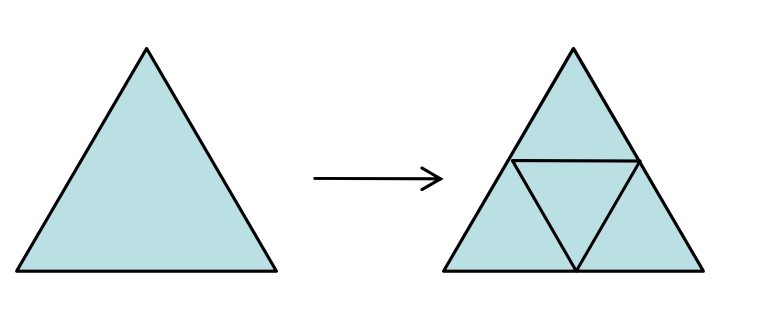
\includegraphics[width=0.3\textwidth]{content/media/sd_loop_split.png}
\caption{Loop Face Split \cite[S. 56 f.]{Standford.24.07.2015}}
\label{fig:sd_loop_split}
\end{figure}

